\documentclass[systemskiss/skiss.tex]{subfiles}

\begin{document}
\section{Bärbar dator}
Den bärbara datorn ska användas för att kommunicera med bilen under körning. Den ska kunna skicka och ta emot styrvärden och kunna agera kontroller när bilen går in i manuellt läge.
\subsection{Översiktlig beskrivning av delsystemet}
\begin{figure}[h]
    \centering
    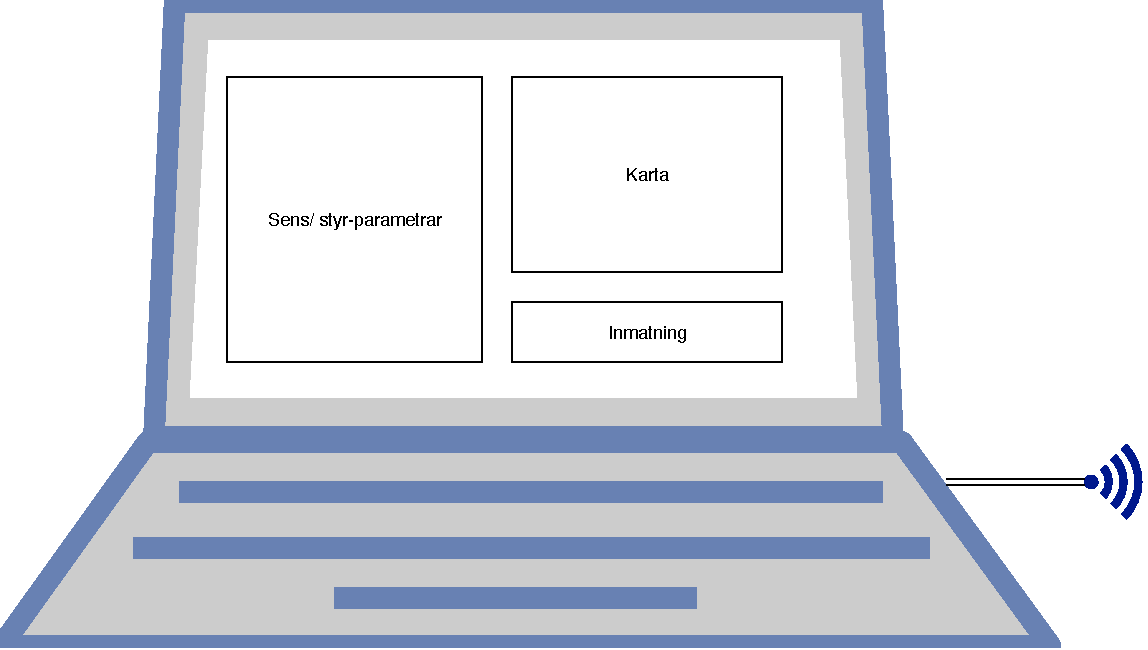
\includegraphics[width=0.6\linewidth]{systemskiss/figures/laptop.pdf}
    \caption{Bild på den bärbara datorn}
    \label{fig:laptopskiss}
\end{figure}
Datorn ska ha någon typ av gränssnitt för att kunna mata in den bana som ska användas under körningen. Datorn ska även kunna visa kartan och kunna visa bilens position i banan.  

\end{document}
